\section{Redefined common words are misread most often, stably, and by many readers}
\label{sec:stable}
\begin{table}[t]\centering\footnotesize\setlength{\tabcolsep}{4pt}
\caption{Reader error without and with the definition text, and AUROC for ranking errors without the definition. $R$ is the proxy score. Freq. is the better of term frequency and term rarity as a ranking score. The definition text is a model-drafted source-based gloss for synthetic, Reddit, and DeFi, and extracted contract wording for CUAD. Rows differ in reader and question construction (Appendix~\ref{app:setting-design}). CUAD is risk-stratified.}
\label{tab:prediction}
\begin{tabular}{@{}llrcccc@{}}\toprule
Corpus & Reader & $n$ & Error, no def. & Error, def. & $R$ AUROC [95\% CI] & Freq.\\\midrule
Synthetic & DeepSeek V4 Flash & 456 & 0.285 & 0.029 & 0.848 [0.811, 0.883] & 0.540\\
Synthetic & GPT-6-astra & 456 & 0.182 & 0.018 & 0.809 [0.763, 0.856] & 0.629\\
Reddit & DeepSeek V4.1 Flash & 1,391 & 0.301 & 0.185 & 0.808 [0.785, 0.835] & 0.544\\
Reddit & GPT-6-astra & 1,391 & 0.146 & 0.119 & 0.720 [0.676, 0.761] & 0.588\\
DeFi & DeepSeek V4.1 Flash & 379 & 0.282 & 0.193 & 0.809 [0.763, 0.856] & 0.510\\
DeFi & GPT-5.6-terra & 379 & 0.230 & 0.148 & 0.792 [0.742, 0.839] & 0.589\\
DeFi & GPT-6-astra & 379 & 0.169 & 0.135 & 0.764 [0.704, 0.815] & 0.603\\
CUAD & GPT-5.6-terra & 1,500 & 0.213 & 0.160 & 0.815 [0.789, 0.840] & 0.507\\
\bottomrule\end{tabular}\end{table}
Table~\ref{tab:prediction} reports how often readers misread. Without the definition, DeepSeek V4 Flash errs on 28.5\% of synthetic questions and GPT-6-astra on 18.2\%. In the contract library, GPT-5.6-terra errs on an estimated 13.2\% of the 6,529 scored questions after reweighting the stratified sample. The exploratory Reddit and DeFi sets give 14.6\% to 30.1\%. With the definition text, error falls in every row, so these errors reflect missing information rather than an inability to answer the question.

\begin{table}[t]\centering\footnotesize\setlength{\tabcolsep}{4pt}
\caption{Contract questions from the validation sample that GPT-5.6-terra answers wrongly without the definition and correctly with it. The usual meaning of each term suggests a broader reading. Percentiles are within the 6,529-question risk index.}
\label{tab:examples}
\begin{tabular}{@{}p{1.5cm}p{3.6cm}p{3.9cm}p{2.9cm}r@{}}\toprule
Term & Local definition & Question (abridged) & Answer implied by the definition & Risk\\\midrule
\emph{Products} & dietary supplements manufactured within the United States & Which products must the endorser have used to give honest findings? & only U.S.-made supplements & 97th\\
\emph{Trademarks} & the trademarks and trade names identified in Exhibit~A & Must the distributor report a confusable third-party name not in Exhibit~A? & report only names listed in Exhibit~A & 99.7th\\
\emph{Term} & the period from the Signing Date to the End Date & During which period must the required insurance stay in force? & from signing to the stated end date, not until termination & 98th\\
\bottomrule\end{tabular}\end{table}

\begin{figure}[t]
\centering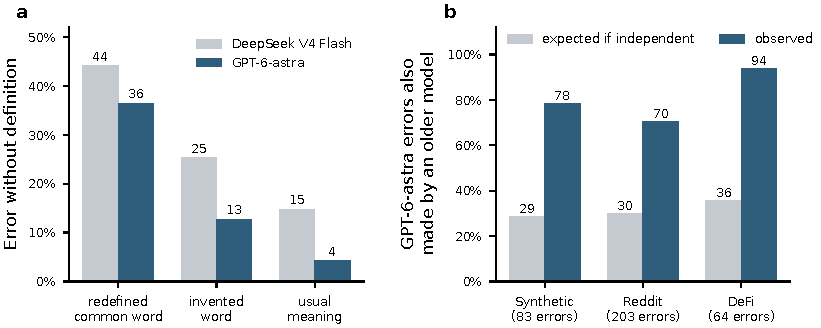
\includegraphics[width=.85\linewidth]{figs/phenomenon.pdf}
\caption{(a) Error without the definition on synthetic questions by designed term class. Familiar words given a new meaning are misread most often. (b) Share of GPT-6-astra's errors that another reader also makes on the same questions, against the share expected if errors were independent, which is the other readers' overall error rate on those questions (for DeFi, the rate at which DeepSeek V4.1 Flash or GPT-5.6-terra errs).}
\label{fig:phenomenon}
\end{figure}

The errors concentrate on familiar words given a new meaning. On synthetic terms whose local meaning conflicts with the usual one, DeepSeek V4 Flash errs on 44.2\% of questions, against 25.3\% on coined words and 14.8\% on words that keep their usual meaning. GPT-6-astra shows the same order, with 36.5\%, 12.7\%, and 4.2\% (Figure~\ref{fig:phenomenon}a). A familiar word misleads more than an unfamiliar one because the reader already has a confident reading of it. Table~\ref{tab:examples} shows three contract cases in which the usual meaning suggests a broader reading than the contract allows.

The errors are also stable. For 761 synthetic questions, DeepSeek V4 Flash gave a greedy answer and ten sampled answers at temperature 1.0. Of the 229 greedy errors, 93 (40.6\%) repeat the same wrong answer in all ten samples, and the majority answer is wrong for 142 (62\%). Majority voting would correct 38\% of greedy errors, but the errors that survive concentrate on redefined common words, where 65\% survive against 43\% on usual-meaning terms. A system that relies on agreement across samples \citep{self-consistency} removes the unstable errors and keeps the ones tied to local meaning.

Errors also overlap strongly across readers. On questions answered by every reader of a corpus, 78\% of GPT-6-astra's synthetic errors are also errors of DeepSeek V4 Flash, 70\% of its Reddit errors are also errors of DeepSeek V4.1 Flash, and 94\% of its DeFi errors are also made by DeepSeek V4.1 Flash or GPT-5.6-terra. If errors were independent, these shares would be 29\%, 30\%, and 36\% (Figure~\ref{fig:phenomenon}b). The readers differ in family and size, so this is not a controlled comparison of model generations, but it shows that the occurrences at risk depend on the text as much as on the model.
